\documentclass[]{article}

\usepackage[utf8]{inputenc}
\usepackage[paperheight=0.7in,paperwidth=1.2in,margin=.1mm]{geometry}
\usepackage{tikz}
\usetikzlibrary{shapes, arrows, calc}
\usepackage{color}

\begin{document}

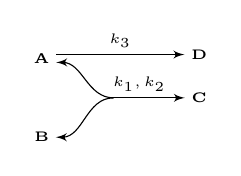
\begin{tikzpicture}[>=latex']
\tiny
\node  at (0, 0)   (A) {$\bf A$};
\node  at (0, -1)  (B) {$\bf B$};
\node  at (2, -.5) (C) {$\bf C$};
\node  at (2, 0.05)   (D) {$\bf D$};
\node  at (1, -.5) (fakeD) {};
\path ($(A.east)+(0,-0.05)$) edge[<-, out=0, in=180] (fakeD);
\path (B) edge[<-, out=0, in=180] (fakeD);
\path ($(fakeD)+(-.1,0)$) edge[->] node[above,xshift=-0.5em] {$k_1,k_2$} (C);
\path ($(A.east)+(0,0.05)$) edge[->] node[above] {$k_3$} (D);
\end{tikzpicture} 
\end{document}
